
\section{例子与计算}

本节中我们将亲手演算一批显式例子，以体会\trBlowup{}如何运作、有何用处，以及如何显式地与它们打交道\footnote{原书此处作「a number of explicit of examples」，当为「a number of explicit examples」之误，径改。——译者注}。\textbf{我们全节都在一个\trField{} $k$ 上工作，并全节约定 $\operatorname{char}k=0$，以免分心。}这些例子与练习大体按论题编排，但并不按重要程度排序。

\textbf{22.4.1.}\ \emph{\trhExample{}：沿原点胀开平面。}\quad 我们先沿原点胀开平面 $\mathbb{A}^2$，看看所得结果与 \S22.1 的讨论相符。取 $x$、$y$ 为 $\mathbb{A}^2$ 上的\trCoordinate。\trBlowup{}是 $\Proj k[x,y,X,Y]$，其中 $xY-yX=0$（此处 $x$ 与 $y$ 的次数为 $0$，而 $X$ 与 $Y$ 的次数为 $1$）。它自然是 $\mathbb{A}^2\times\mathbb{P}^1$ 的一个\trClosedSubscheme，由 $xY-yX=0$ 切出（以 $\mathbb{P}^1$ 上的射影\trCoordinate{} $X$、$Y$ 表出）。我们考虑 $\mathbb{P}^1$ 上通常的那两个片：$[X,Y]=[s,1]$ 与 $[1,t]$。第一片给出 $\Spec k[x,y,s]/(sy-x)$，第二片给出 $\Spec k[x,y,t]/(y-xt)$。注意二者都\trSmooth：前者是 $\Spec k[y,s]\cong\mathbb{A}^2$，而后者是 $\Spec k[x,t]\cong\mathbb{A}^2$。

现在我们来描述\trExceptionalDivisor。先考虑第一个（$s$）片。\trIdeal{}由 $(x,y)$ 生成，而在我们本片的 $y$、$s$ 坐标之下它就是 $(ys,y)=(y)$\footnote{原书此处作「ys-coordinates」，当为「y、s-coordinates」之误，径改。——译者注}，确实是\trPrincipal{}的。于是在这一片上，\trExceptionalDivisor{}由 $y$ 生成。类似地，在第二片上，\trExceptionalDivisor{}由 $x$ 切出。（这可能有点令人迷惑，但其实并无矛盾！）这一显式描述，将有助于我们演算下面的一些例子。

\textbf{22.4.A.（练习）}\quad 设 $p$ 是 $\mathbb{P}^2$ 的一个 $k$-\trValuedPoint。请具体构造出 $\mathrm{Bl}_p\mathbb{P}^2$ 与\trHirzebruchSurface{} $\mathbb{F}_1=\mathbb{P}_{\mathbb{P}^1}\bigl(\OO_{\mathbb{P}^1}\oplus\OO_{\mathbb{P}^1}(1)\bigr)$（\mbox{例~17.2.6}）之间的一个\trIsomorphism。（映射 $\mathrm{Bl}_p\mathbb{P}^2\to\mathbb{P}^1$ 非正式地说相应于「把一个点送到连接它与原点的那条直线」这一操作。不必害怕：你完全可以借显式摆弄\trCoordinate{}来完成。）

\textbf{22.4.2. 解消\trSingularPoint。}

\textbf{22.4.3.}\ \emph{一条\trNode{}\trCurve{}的\trProperTransform}（图~\ref{fig:resolving-curve-singularities}）。\quad （思考这道练习时，你或许愿意翻到图~\ref{fig:normalization-nodal-cubic} 对照着看。）接下来考虑平面 $\mathbb{A}^2$ 内的\trCurve{} $y^2=x^3+x^2$（\trNode{}三次曲线，见\mbox{练习~22.3.B}）。我们在原点处作\trBlowup，并计算这条\trCurve{}的\trTotalTransform{}与\trProperTransform。（由\mbox{\trBlowupClosureLemma~22.2.7}，后者正是这条\trNode{}\trCurve{}在原点处的\trBlowup。）在第一片中，我们得到 $y^2-s^2y^2-s^3y^3=0$。它可以分解因子：我们得到带重数 $2$ 的\trExceptionalDivisor{} $y$，以及\trCurve{} $1-s^2-s^3y=0$。你可以轻松验证\trProperTransform{}是\trRegular{}的。另外，请注意\trProperTransform{} $\bar{C}$ 与\trExceptionalDivisor{}相交于两点 $s=\pm 1$。这相应于原点处的两个\trTangentLine{}方向（因为 $s=x/y$）。（第二片请你自行完成。）

\begin{figure}[htbp]
\centering
\begin{tikzpicture}[scale=0.9,line width=0.8pt]
  \draw (0,1.55) -- (1.5,1.55) -- (2.0,2.7) -- (0.5,2.7) -- cycle;
  \draw (2.55,1.55) -- (4.05,1.55) -- (4.55,2.7) -- (3.05,2.7) -- cycle;
  \draw (5.1,1.55) -- (6.6,1.55) -- (7.1,2.7) -- (5.6,2.7) -- cycle;
  \node at (-1.15,2.15) {$\mathrm{Bl}_{(0,0)}\mathbb{A}^2$};
  \draw[line width=1.3pt] (1.15,1.75) -- (1.15,2.55);
  \node at (0.85,2.6) {$\mathrm{E}$};
  \draw (1.6,1.85) .. controls (1.0,1.95) and (0.9,2.35) .. (1.25,2.42)
        .. controls (1.5,2.46) and (1.55,2.22) .. (1.72,2.12);
  \node at (1.5,1.98) {$\widetilde{C}$};
  \draw[line width=1.3pt] (3.7,1.75) -- (3.7,2.55);
  \node at (3.42,2.6) {$\mathrm{E}$};
  \draw (3.0,1.9) .. controls (3.55,1.98) and (3.55,2.25) .. (3.95,2.32)
        .. controls (4.15,2.36) and (4.25,2.32) .. (4.4,2.4);
  \node at (4.2,2.1) {$\widetilde{C}$};
  \draw[line width=1.3pt] (6.25,1.75) -- (6.25,2.55);
  \node at (5.97,2.6) {$\mathrm{E}$};
  \draw (6.95,2.5) .. controls (6.45,2.44) and (6.25,2.3) .. (6.25,2.15)
        .. controls (6.25,2.0) and (6.5,1.9) .. (6.8,1.85);
  \node at (6.72,2.32) {$\widetilde{C}$};
  \draw[gray!75,->] (1.35,1.45) -- (1.35,-0.2);
  \draw[gray!75,->] (3.9,1.45) -- (3.9,-0.2);
  \draw[gray!75,->] (6.45,1.45) -- (6.45,-0.2);
  \draw (0,-1.35) -- (1.5,-1.35) -- (2.0,-0.2) -- (0.5,-0.2) -- cycle;
  \draw (2.55,-1.35) -- (4.05,-1.35) -- (4.55,-0.2) -- (3.05,-0.2) -- cycle;
  \draw (5.1,-1.35) -- (6.6,-1.35) -- (7.1,-0.2) -- (5.6,-0.2) -- cycle;
  \node at (-1.15,-0.75) {$\mathbb{A}^2$};
  \draw (0.5,-0.55) .. controls (0.8,-0.95) and (1.35,-0.95) .. (1.5,-0.6)
        .. controls (1.6,-0.36) and (1.28,-0.3) .. (1.08,-0.5)
        .. controls (0.93,-0.65) and (0.78,-0.65) .. (0.7,-0.48)
        .. controls (0.63,-0.32) and (0.82,-0.16) .. (1.08,-0.18);
  \node at (1.75,-0.55) {$C$};
  \draw (2.95,-1.1) .. controls (3.35,-0.6) and (3.9,-0.42) .. (4.45,-0.35);
  \node at (4.25,-0.58) {$C$};
  \draw (5.95,-0.75) .. controls (6.4,-0.46) and (6.75,-0.46) .. (6.95,-0.62);
  \draw (5.95,-0.75) .. controls (6.4,-1.04) and (6.7,-1.04) .. (6.85,-0.86);
  \node at (6.62,-0.75) {$C$};
  \node at (1.0,-1.75) {$\S$22.4.3};
  \node at (3.55,-1.75) {练习~22.4.B};
  \node at (6.1,-1.75) {练习~22.4.C};
\end{tikzpicture}
\caption{解消\trCurve\trSingularPoint。（依原书手绘图重绘。）}\label{fig:resolving-curve-singularities}
\end{figure}

\textbf{22.4.B.（练习，图~\ref{fig:resolving-curve-singularities}）}\quad 描述 $\mathrm{Bl}_{(0,0)}\mathbb{A}^2$ 中由 $y=x^2-x$ 给出的\trCurve{} $C$ 的\trTotalTransform{}与\trProperTransform{}二者。证明 $C$ 的\trProperTransform{}\trIsomorphic{}于 $C$。请把 $C$ 的\trProperTransform{}与\trExceptionalDivisor{} $\mathrm{E}$ 的\trIntersection{}解读为 $C$ 在原点处的斜率。

\textbf{22.4.C.（练习：胀开一条尖点平面曲线，参看\mbox{练习~10.7.F}）}\quad 描述 $\mathrm{Bl}_{(0,0)}\mathbb{A}^2$ 中由 $y^2=x^3$ 给出的\trCusp{}\trCurve{} $C$ 的\trProperTransform。证明它是\trRegular{}的。证明 $C$ 的\trProperTransform{}与\trExceptionalDivisor{} $\mathrm{E}$ 相交于一点，且在该点与 $\mathrm{E}$ 相切。

上面两道练习是一个重要的\trSingularPoint{}序列中的头几个，我们现在就来讨论这个序列。

\textbf{22.4.D.（练习：解消 $A_n$ \trCurve\trSingularPoint）}\quad 解消 $\mathbb{A}^2$ 中的\trSingularPoint $y^2=x^{n+1}$：先在其\trSingularPoint{}处作\trBlowup，然后考虑其\trProperTransform，并决定下一步该做什么。

\textbf{22.4.4.}\ \emph{迈向 $A_n$ \trCurve\trSingularPoint{}的一个定义。}\quad 你会注意到，你对\mbox{练习~22.4.D} 的解答只依赖于该\trSingularPoint{}在原点处的「幂级数展开」，而不依赖于具体的方程。例如，把 \S22.4.3 与\mbox{练习~22.4.D} 的 $n=1$ 情形相比较，你会发现二者「基本相同」。我们将在\mbox{定义~28.2.C} 中把这一点说精确。

\textbf{22.4.E.（练习：\mbox{练习~22.4.F} 的热身）}\quad 在原点处胀开\trCone{}面 $z^2=x^2+y^2$（图~\ref{fig:cone-picture}）的\trCone{}点。证明所得曲面是\trRegular{}的。证明\trExceptionalDivisor{}\trIsomorphic{}于 $\mathbb{P}^1$。（评注：你可以验证，这个 $\mathbb{P}^1$ 的\trNormalBundle{}并不是 $\OO_{\mathbb{P}^1}(-1)$——在光滑曲面上胀开一点时才是如此；见 \S22.3.4——它是 $\OO_{\mathbb{P}^1}(-2)$。这岂不与\mbox{练习~22.3.D}(b) 矛盾？）

\textbf{22.4.F.（练习：解消 $A_n$ \trSurface\trSingularPoint）}\quad 解消 $\mathbb{A}^3$ 中的\trSingularPoint $z^2=y^2+x^{n+1}$：先在其\trSingularPoint{}处作\trBlowup，然后考虑其\trProperTransform，并决定下一步该做什么。（与这一\trSingularPoint\trAnalyticallyIsomorphic（analytically isomorphic）的 $k$-\trSurface\trSingularPoint，称作一个 $A_n$ \textbf{\trSurface\trSingularPoint}（surface singularity）。例如，图~\ref{fig:cone-picture} 中所示的那个锥便是一个 $A_1$ \trSurface\trSingularPoint。我们将在\mbox{练习~28.2.C} 中把这件事说精确。）这道练习做起来有些费时，但回报丰厚：它表明你确实可以徒手解消\trSingularPoint。

\textbf{22.4.5.}\ \emph{\trhRemark{}：ADE \trSurface\trSingularPoint{}与\trDynkinDiagram}（见图~\ref{fig:ade-dynkin}）。\quad 一个与 $z^2=x^2y+y^{n-1}$（相应地，$z^2=x^3+y^4$、$z^2=x^3+xy^3$、$z^2=x^3+y^5$）\trAnalyticallyIsomorphic{}的 $k$-\trSingularPoint，称作一个 $D_n$ \trSurface\trSingularPoint（相应地，$E_6$、$E_7$、$E_8$ \trSurface\trSingularPoint）\footnote{原书此处作「is a called」，当为「is called」之误，径改。——译者注}。我们将在\mbox{练习~28.2.C} 中把这件事说精确，届时你将能够猜出相应\trCurve\trSingularPoint{}的定义。若你像\mbox{练习~22.4.F} 那样，通过在\trSingularPoint{}处逐一作\trBlowup{}来（以极小方式）将这些曲面各自\trDesingularization，并审视\trExceptionalDivisor{}的排布（各个\trExceptionalDivisor{}以及它们如何相交），你将会发现相应的\textbf{\trDynkinDiagram}（Dynkin diagram）。更精确地说：若你造出这样一张图——顶点相应于诸\trExceptionalDivisor，而当两个除子相交时便用一条边把相应顶点连起来——你将会找到相应\trDynkinDiagram{}的基础图。这是好几个非常漂亮的故事的开端；其中之一可以让你先睹为快，见\mbox{注记~27.3.7}。

\begin{figure}[htbp]
\centering
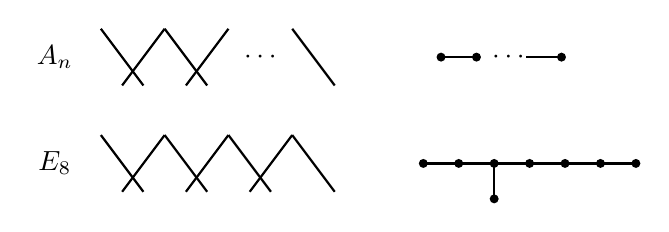
\begin{tikzpicture}[scale=0.9,line width=0.8pt]
  \node at (-0.85,0.55) {$A_n$};
  \draw (-0.2,0.95) -- (0.4,0.15);
  \draw (0.1,0.15) -- (0.7,0.95);
  \draw (0.7,0.95) -- (1.3,0.15);
  \draw (1.0,0.15) -- (1.6,0.95);
  \node at (2.05,0.55) {$\cdots$};
  \draw (2.5,0.95) -- (3.1,0.15);
  \fill (4.6,0.55) circle (1.8pt);
  \draw (4.6,0.55) -- (5.1,0.55);
  \fill (5.1,0.55) circle (1.8pt);
  \node at (5.55,0.55) {$\cdots$};
  \draw (5.8,0.55) -- (6.3,0.55);
  \fill (6.3,0.55) circle (1.8pt);
  \node at (-0.85,-0.95) {$E_8$};
  \draw (-0.2,-0.55) -- (0.4,-1.35);
  \draw (0.1,-1.35) -- (0.7,-0.55);
  \draw (0.7,-0.55) -- (1.3,-1.35);
  \draw (1.0,-1.35) -- (1.6,-0.55);
  \draw (1.6,-0.55) -- (2.2,-1.35);
  \draw (1.9,-1.35) -- (2.5,-0.55);
  \draw (2.5,-0.55) -- (3.1,-1.35);
  \fill (4.35,-0.95) circle (1.8pt);
  \draw (4.35,-0.95) -- (4.85,-0.95);
  \fill (4.85,-0.95) circle (1.8pt);
  \draw (4.85,-0.95) -- (5.35,-0.95);
  \fill (5.35,-0.95) circle (1.8pt);
  \draw (5.35,-0.95) -- (5.85,-0.95);
  \fill (5.85,-0.95) circle (1.8pt);
  \draw (5.85,-0.95) -- (6.35,-0.95);
  \fill (6.35,-0.95) circle (1.8pt);
  \draw (6.35,-0.95) -- (6.85,-0.95);
  \fill (6.85,-0.95) circle (1.8pt);
  \draw (6.85,-0.95) -- (7.35,-0.95);
  \fill (7.35,-0.95) circle (1.8pt);
  \draw (5.35,-0.95) -- (5.35,-1.45);
  \fill (5.35,-1.45) circle (1.8pt);
\end{tikzpicture}
\caption{一些 ADE \trSurface\trSingularPoint{}的解消中的\trExceptionalDivisor，以及它们相应的对偶图（见\mbox{注记~22.4.5}）。（依原书手绘图重绘。）}\label{fig:ade-dynkin}
\end{figure}

\textbf{22.4.6.}\ \emph{\trhRemark{}：\trResolutionOfSingularities。}\quad \trHironaka{}的\trResolutionOfSingularities{}定理蕴含：一般地，「通过胀开\trSingularLocus{}来解消\trSingularPoint」这一想法在\trCharacteristic{} $0$ 下能够成功（见 [Hir] 与 [Ko2]）。（维数 $1$ 的情形将在 \S28.4.4 中证明，维数 $2$ 的情形将在 \S28.6.4 中讨论。）类似的陈述在正\trCharacteristic{}下是否为真尚不可知（维数至多 $3$ 的情形除外；见 [CP]），但\trDeJong{}的\textbf{\trAlterationTheorem}（Alteration Theorem）[dJ] 给出了一个对大多数应用而言足够好的结果：它并不给出从某个正则之物到 $X$ 的\trBirational\trProper{}映射 $\widetilde{X}\to X$，而是给出一个来自某个正则之物的\trProper{}映射，其为一般有限的（并且相应的函数域扩张是可分的）。

下面是一些与\trResolutionOfSingularities{}有关的其他练习。

\textbf{22.4.G.（练习）}\quad 胀开正则概形的一个非既约\trSubscheme{}可能给你带来\trSingular{}之物，本例即是一例。请描述 $\Spec k[x,y]=\mathbb{A}^2$ 中\trClosedSubscheme{} $V(y,x^2)$ 的\trBlowup。证明你得到一个 $A_1$ \trSurface\trSingularPoint。

\textbf{22.4.H.（练习）}\quad 对\trTacnode{}（见\mbox{练习~10.7.G} 与\mbox{定义~28.2.2}）$y^2=x^4$ \trDesingularization：不像\mbox{练习~22.4.D} 那样分两步走，而是一步到位——胀开 $(y,x^2)$。

\textbf{22.4.I.（练习：借一个出乎意料的胀开解消\trSingularPoint）}\quad 设 $Y$ 是\trCone{}面 $x^2+y^2=z^2$，而 $X$ 是 $Y$ 上由 $x=0$、$y=z$ 切出的直线。证明 $\mathrm{Bl}_X\,Y$ 是\trRegular{}的。（此处我们是在胀开一个不是\trEffectiveCartierDivisor{}的余维数 $1$ 轨迹；见\mbox{问题~13.1.3}。但在离开\trCone{}点的地方它是\trEffectiveCartierDivisor，所以你应当预期：你的答案在离开\trCone{}点之处是\trIsomorphism。）

\textbf{22.4.7.}\ \emph{函数在\trRegular{}点处的\trMultiplicity。}\quad 为了提出\mbox{练习~22.4.J}，我们引入一个有用的概念。若 $f$ 是\trLocally\trNoetherian{}\trScheme{} $X$ 上的一个函数，则它在\trRegular{}点 $p$ 处的\textbf{\trMultiplicity}（multiplicity at a regular point），是使 $f$ 落入局部环 $\OO_{X,p}$ 中\trMaximalIdeal{}的 $m$ 次幂之内的最大的 $m$。例如，若 $f\neq 0$，则 $V(f)$ 在 $p$ 处\trSingular{}当且仅当 $m>1$。（你明白这是为什么吗？）

\textbf{22.4.J.（练习）}\quad 证明：在原点处作\trBlowup{}时，$\mathbb{A}^n$ 的\trSubscheme{} $Z$ 的\trTotalTransform{}中\trExceptionalDivisor{}的\trMultiplicity，等于 $Z$ 的一个定义方程（在原点处）的最小\trMultiplicity。（例如，对上面的\trNode{}\trCurve{}与\trCusp{}\trCurve{}的情形，即\mbox{例~22.4.3} 与\mbox{练习~22.4.C}，\trExceptionalDivisor{}都以重数 $2$ 出现。）警示：在着手求解之前，你需要先把这个问题说精确。

\textbf{22.4.8. 解消\trRationalMap。}

\textbf{22.4.K.（练习：借胀开理解\trBirational\trRationalMap{} $\mathbb{P}^2\dashrightarrow\mathbb{P}^1\times\mathbb{P}^1$）}\quad 设 $p$、$q$ 是 $\mathbb{P}^2$ 中两个不同的 $k$-点，并设 $r$ 是 $\mathbb{P}^1\times\mathbb{P}^1$ 的一个 $k$-点。请描述一个\trIsomorphism{} $\mathrm{Bl}_{\{p,q\}}\mathbb{P}^2\overset{\sim}{\longleftrightarrow}\mathrm{Bl}_r\,\mathbb{P}^1\times\mathbb{P}^1$。（可能的提示：考虑过 $p$ 的直线 $\ell$ 与过 $q$ 的直线 $m$；这样一对直线的选取，相应于 $\mathbb{P}^1\times\mathbb{P}^1$ 的一个点。$\mathbb{P}^2$ 中不在直线 $\overline{pq}$ 上的一个点 $s$，给出一对直线 $(\overline{ps},\overline{qs})$，即 $\mathbb{P}^1\times\mathbb{P}^1$ 的一个点。反之，选取一对直线 $(\ell,m)$，只要 $\ell$ 与 $m$ 都不是直线 $\overline{pq}$，便给出一个点 $s=\ell\cap m\in\mathbb{P}^2$。这就描述了一个\trBirational\trRationalMap{} $\mathbb{P}^2\dashrightarrow\mathbb{P}^1\times\mathbb{P}^1$。\mbox{练习~22.4.A} 与此有关。）

\mbox{练习~22.4.K} 是接下来两道练习所探究的那个一般现象的一个例子。

\textbf{22.4.L.（较难而有用的练习：胀开解消到射影空间之\trRationalMap{}的\trBaseLocus）}\quad 设我们有一个\trScheme{} $Y$、一个\trInvertibleSheaf{} $\mathscr{L}$，以及 $\mathscr{L}$ 的若干个\trSection{} $s_0,\dots,s_n$（一个\trLinearSystem，\mbox{定义~15.2.1}）。那么，在由 $s_0=\cdots=s_n=0$ 切出的\trClosedSubscheme{} $X$（该\trLinearSystem{}的\trBaseLocus）之外，这些\trSection{}给出一个到 $\mathbb{P}^n$ 的\trMorphism。证明：这个\trMorphism{}可以唯一地延拓为一个\trMorphism{} $\mathrm{Bl}_X\,Y\to\mathbb{P}^n$，且这个\trMorphism{}相应于\trInvertibleSheaf{} $(\beta^*\mathscr{L})(-\mathrm{E}_X\,Y)$，其中 $\beta\colon\mathrm{Bl}_X\,Y\to Y$ 是\trBlowup{}\trMorphism。换言之：「把概形论\trBaseLocus{}胀开，便解消了这个\trRationalMap」。提示：只须考虑 $Y$ 的一个使 $\mathscr{L}$ 平凡的\trAffine\trOpenSubset{}即可。唯一性或可借用\mbox{练习~11.3.G}。

\textbf{22.4.9.}\ \emph{\trhRemark。}\quad
（i）\mbox{练习~22.4.L} 立即蕴含：胀开可以用来解消到射影概形的\trRationalMap{} $Y\dashrightarrow Z\hookrightarrow\mathbb{P}^n$。

（ii）下面的解读富有启发。$Y$ 上的\trLinearSystem{}拉回为 $\mathrm{Bl}_X\,Y$ 上的\trLinearSystem，而 $Y$ 上\trLinearSystem{}的\trBaseLocus{}拉回为 $\mathrm{Bl}_X\,Y$ 上的\trBaseLocus。$\mathrm{Bl}_X\,Y$ 上的\trBaseLocus{}正是 $\mathrm{E}_X\,Y$，一个\trEffectiveCartierDivisor。由于 $\mathrm{E}_X\,Y$ 不仅\trLocallyPrincipal，而且还局部地是个\trNonZerodivisor，故可以把它从诸 $\beta^*s_i$ 中「除出去」（由此得到 $(\beta^*\mathscr{L})(-\mathrm{E}_X\,Y)$ 的一个\trSection），从而去除\trBaseLocus，留下一个\trBasePointFree{}的\trLinearSystem。（借\trUniversalProperty{}可以把这件事说精确：这是 $Y$ 的能够去除\trBaseLocus{}的最小「修改」。）若 $X$ 本来就是\trCartier{}的（例如，当 $Y$ 是\trRegular{}\trPureDimensional{}\trCurve{}时，任何非平凡的\trLinearSystem{}都必然如此），那么我们只须「把 $X$ 除出去」便能去除\trBaseLocus。

（iii）你或许愿意重访\mbox{练习~19.7.C}，并用\mbox{练习~22.4.L} 的语言来解读它。

\textbf{22.4.10.}\ \emph{若干例子。}\quad
（i）由 $[x_0,\cdots,x_n]\dashrightarrow[x_1,\cdots,x_n]$ 给出、定义在 $p=[1,0,\cdots,0]$ 之外的\trRationalMap{} $\mathbb{P}^n\dashrightarrow\mathbb{P}^{n-1}$，可以通过胀开 $p$ 来解消。于是，由\mbox{\trBlowupClosureLemma~22.2.7}，若 $Y$ 是 $\mathbb{P}^n$ 的任一局部闭\trSubscheme，那么一旦胀开 $Y$ 中的 $p$，我们便可投射到 $\mathbb{P}^{n-1}$，而给出这个到 $\mathbb{P}^{n-1}$ 之映射的\trInvertibleSheaf{}是（稍显不正式地说）$\beta^*(\OO_{\mathbb{P}^n}(1))\otimes\OO(-\mathrm{E}_p\,Y)$。

（ii）考虑三个变元的两个一般齐次三次函数 $C_1$ 与 $C_2$，它们给出 $\mathbb{P}^2$ 中两条三次曲线。二者都\trSmooth{}（由\mbox{\trBertini{}定理~13.4.2}），并相交于九个点 $p_1,\dots,p_9$（利用我们的\trStandingHypothesis：在代数闭域上工作）。于是 $[C_1,C_2]$ 给出一个\trRationalMap{} $\mathbb{P}^2\dashrightarrow\mathbb{P}^1$。为了解消这个\trRationalMap，我们胀开 $p_1,\dots,p_9$。所得结果（一般地）是一个\emph{\trEllipticFibration}（elliptic fibration）$\mathrm{Bl}_{\{p_1,\dots,p_9\}}\mathbb{P}^2\to\mathbb{P}^1$。（这绝算不上一个完整的论证，甚至算不上一个精确的陈述。）

（iii）取定 $\mathbb{P}^2$ 中六个一般的点 $p_1,\dots,p_6$。在这些点上消失的三次函数构成一个四维\trVectorSpace，而且它们恰好概形论地消失且仅消失于这些点。这就给出一个\trRationalMap{} $\mathbb{P}^2\dashrightarrow\mathbb{P}^3$，通过胀开这六个点可以将其解消。所得的\trMorphism{}结果是一个\trClosedEmbedding，而它在 $\mathbb{P}^3$ 中的像是一个（光滑的）三次曲面。这就是那个著名的事实：平面在六个一般点处的胀开可以表示为 $\mathbb{P}^3$ 中的一个（光滑）三次曲面。（同样，这个论证也无意求全。）更精确、更完整的讨论见 \S27.3.5。

在合理的情形下，\mbox{练习~22.4.L} 有一个借\trRationalMap{}之图像的解读。

\textbf{22.4.M.（练习）}\quad 设 $s_0,\dots,s_n$ 是\trIntegral\trScheme{} $X$ 上某个\trInvertibleSheaf{} $\mathscr{L}$ 的\trSection，不全为 $0$。由\mbox{注记~15.2.5}，这些资料给出一个\trRationalMap{} $\phi\colon X\dashrightarrow\mathbb{P}^n$。请在 $\phi$ 的图像（\S11.3.4）与 $\mathrm{Bl}_{V(s_0,\dots,s_n)}\,X$ 之间给出一个\trIsomorphism。（你的论证将不需要在\trField{} $k$ 上工作；它在一般情形下都成立。）

你或许会乐于探究前一个想法，亲手演算一下\trCremona{}变换 $\mathbb{P}^2\dashrightarrow\mathbb{P}^2$（\mbox{练习~7.5.J}）如何能借\trRationalMap{} $[x,y,z]\dashrightarrow[1/x,\,1/y,\,1/z]$ 的图像来解读。

\textbf{22.4.N.}\ \hard\ \textbf{（练习）}\quad 解消从\trQuadricSurface{}上的\trCone{}出发、到射影直线的\trRationalMap
\[
\Spec k[w,x,y,z]/(wz-xy)\mathrel{\overset{[w,x]}{\dashrightarrow}}\mathbb{P}^1.
\]
设 $X$ 是所得的\trVariety，而 $\pi\colon X\to\Spec k[w,x,y,z]/(wz-xy)$ 是到\trQuadricSurface{}上的那个\trCone{}的\trProjection。证明：$\pi$ 在离开\trCone{}点处是\trIsomorphism，且\trCone{}点的原像\trIsomorphic{}于 $\mathbb{P}^1$（从而具有余维数 $2$，故不同于单纯胀开\trCone{}点所得的那个解消）。可能的提示：若 $Q$ 是 $\mathbb{P}^3$ 中由 $wz-xy=0$ 切出的\trQuadricSurface，则把这个\trRationalMap{}分解为 $\Spec k[w,x,y,z]/(wz-xy)\setminus\{0\}\to Q$（参看\mbox{练习~9.3.N}），继以\trIsomorphism{} $Q\overset{\sim}{\longrightarrow}\mathbb{P}^1\times\mathbb{P}^1$（\mbox{例~10.6.2}），再投射到其中一个因子。

这是一个\textbf{\trSmallResolution}（small resolution）的例子。（\trSmallResolution{} $X\to Y$ 是这样一种解消：$Y$ 中纤维具有维数 $r$ 的点的轨迹，其余维数大于 $2r$。我们不会再以任何实质的方式用到这个概念。警示：这是\trIntersectionHomology（intersection homology）中所用的「小解消」定义；在\trMinimalModelProgram{}中，小解消则指在余维数 $1$ 处为\trIsomorphism{}的解消。所以请留意你所读内容的语境。）注意，这个对态射的解消涉及胀开\trBaseLocus{} $w=x=0$，它是以\trQuadricSurface $wz=xy$ 上某条直线为底的\trCone。我们是在胀开一个\trEffective\trWeilDivisor，由于这个胀开不是\trIsomorphism，它必然不是\trCartier{}的。在\mbox{练习~13.1.E} 中我们曾看到 $(w,x)$ 不是\trPrincipal{}的，而这里我们看到 $(w,x)$ 甚至不是\trLocallyPrincipal{}的。本质上由\mbox{练习~15.5.N}，$V(w,x)$ 甚至不能充当任何\trLocallyPrincipal{}除子的\trSupport。

\textbf{22.4.11.}\ \emph{\trhRemark{}：互不同构的小解消。}\quad 如果你改为解消映射 $[w,y]$，你将得到一个看起来相像的小解消
\[
\pi'\colon X'\longrightarrow\Spec k[w,x,y,z]/(wz-xy)
\]
（它在离开原点处是\trIsomorphism，而原点之上的纤维是 $\mathbb{P}^1$）。但它有所不同！更精确地说：不存在使下图交换的\trMorphism{} $X\to X'$\footnote{原书此处作「making the following the diagram commute」，当为「making the following diagram commute」之误，径改。——译者注}
\[
\begin{tikzcd}
X \ar[rr] \ar[dr,"\pi"'] && X' \ar[dl,"\pi'"] \\
& \Spec k[w,x,y,z]/(wz-xy) &
\end{tikzcd}
\]
\trBirational\trRationalMap{} $X\dashrightarrow X'$ 称作\textbf{\trAtiyahFlop}（Atiyah flop），[At1]。

\textbf{22.4.12.}\ \emph{\trBirational\trRationalMap{}的分解。}\quad 在结束关于\trRationalMap{}之解消的讨论之际，我们指出：正如\trHironaka{}定理断言，在\trCharacteristic{} $0$ 下，人们可以沿光滑\trSubvariety{}的\trBlowup{}序列解消\trVariety{}的一切\trSingularPoint（\S22.4.6），\emph{\trWeakFactorizationTheorem}（Weak Factorization Theorem）（首由 Włodarczyk 证明 [Wl]）同样断言：\trCharacteristic{} $0$ 下任意两个\trBirational{}的\trVariety{} $X$ 与 $Y$，都可以借沿光滑\trSubvariety{}的胀开与「收缩」联系起来。更精确地说：存在\trVariety
\[
X_0,\ \dots,\ X_n,\ X_{01},\ \dots,\ X_{(n-1)n}
\]
（其中 $X_0=X$、$X_n=Y$），并存在\trMorphism{} $X_{i(i+1)}\to X_i$ 与 $X_{i(i+1)}\to X_{i+1}$（$0\le i<n$），它们都是光滑\trSubvariety{}的胀开。

\textbf{22.4.13. 胀开与线丛。}

\textbf{22.4.O.（练习：推广\mbox{练习~20.2.D}）}\quad 设 $X$ 是 $k$ 上的一张正则射影曲面，$p$ 是一个 $k$-\trValuedPoint。令 $\beta\colon\mathrm{Bl}_pX\to X$ 为\trBlowup{}\trMorphism，并令 $\mathrm{E}=\mathrm{E}_pX$ 为\trExceptionalDivisor。考虑\eqref{eq:excision-class-groups} 的那个\trExactSequence
\[
\mathbb{Z}\mathrel{\xrightarrow{\ \gamma\colon 1\mapsto[\mathrm{E}]\ }}\mathrm{Pic}(\mathrm{Bl}_pX)\mathrel{\xrightarrow{\ \alpha\ }}\mathrm{Pic}(\mathrm{Bl}_pX\setminus\mathrm{E})\longrightarrow 0
\]
（严格说来，\eqref{eq:excision-class-groups} 中 $\mathrm{Pic}$ 被换成了 $\mathrm{Cl}$。但由于正则局部环都是\trUFD{}（\S13.8.5），依\mbox{命题~15.4.16}，此情形下 $\mathrm{Pic}=\mathrm{Cl}$。）注意 $\mathrm{Bl}_pX\setminus\mathrm{E}=X\setminus p$。证明 $\mathrm{Pic}(X\setminus p)=\mathrm{Pic}\,X$。证明 $\beta^*\colon\mathrm{Pic}\,X\to\mathrm{Pic}\,\mathrm{Bl}_pX$ 给出 $\alpha$ 的一个截面。用 \S22.3.4 证明 $\OO_{\mathrm{Bl}_pX}(\mathrm{E})|_{\mathrm{E}}\cong\OO_{\mathrm{E}}(-1)$\footnote{原书此处作「$\OO_X(E)|_E$」，当为「$\OO_{\mathrm{Bl}_pX}(E)|_E$」之误（$\mathrm{E}$ 是胀开 $\mathrm{Bl}_pX$ 上的除子，本练习下文亦作 $\OO_{\mathrm{Bl}_pX}(\mathrm{E})$），径改。——译者注}（于是，用第 20 章的语言，$\mathrm{E}$ 是一条 $(-1)$-曲线，\mbox{定义~20.2.8}），并由此证明 $\gamma$ 是一个\trInjection。结论：$\mathrm{Pic}\,\mathrm{Bl}_pX\cong\mathrm{Pic}\,X\oplus\mathbb{Z}$。请描述如何由 $\mathrm{N}^1_{\mathbb{Q}}(X)$ 上的相交矩阵求出 $\mathrm{N}^1_{\mathbb{Q}}(\mathrm{Bl}_pX)$ 上的相交矩阵。

\textbf{22.4.P.（练习）}\quad 设 $D$ 是 $X$ 上的一个\trEffectiveCartierDivisor{}（一条\trCurve）。令 $\operatorname{mult}_pD$ 为 $D$ 在 $p$ 处的\trMultiplicity{}（\mbox{练习~22.4.J}），并令 $D^{\mathrm{pr}}$ 为 $D$ 的\trProperTransform。证明：作为\trEffectiveCartierDivisor，有 $\beta^*D=D^{\mathrm{pr}}+(\operatorname{mult}_pD)\mathrm{E}$。更精确地，证明：$D^{\mathrm{pr}}$ 的局部方程与 $\mathrm{E}$ 的局部方程的 $(\operatorname{mult}_pD)$ 次幂二者的乘积，正是 $\beta^*D$ 的局部方程，从而（i）$\beta^*D$ 是一个\trEffectiveCartierDivisor，且（ii）$\beta^*\OO_X(D)\cong\OO_{\mathrm{Bl}_pX}(D^{\mathrm{pr}})\otimes\OO_{\mathrm{Bl}_pX}(\mathrm{E})^{\otimes(\operatorname{mult}_pD)}$。（\mbox{提示~20.2.7} 中的方程 $\ell=e+m$ 便是其一个特例。）

\textbf{22.4.14.}\ \emph{胀开之下典范线丛的变化。}\quad 作为「\trCanonical{}线丛在胀开之下如何变化」的动机，考虑胀开 $\beta\colon\mathrm{Bl}_{(0,0)}\mathbb{A}^2\to\mathbb{A}^2$。为方便计，令 $X=\mathrm{Bl}_{(0,0)}\mathbb{A}^2$、$Y=\mathbb{A}^2$。我们将用\mbox{练习~21.4.A} 来关联 $\beta^*\mathscr{K}_Y$ 与 $\mathscr{K}_X$。

我们在 $(0,0)$ 附近为 $\mathscr{K}_Y$ 选取一个生成元：$\mathrm{d}x\wedge\mathrm{d}y$。（事实上，它在 $\mathbb{A}^2$ 上处处都是 $\mathscr{K}_Y$ 的生成元，但为了便于推广，我们指出：要紧的只是它是 $(0,0)$ 处的生成元，从而由几何\trNakayama{}引理（\mbox{练习~14.3.D}）它也是 $(0,0)$ \emph{附近}的生成元。）把它拉回到 $X$ 上时，我们可以把它解读为 $\mathscr{K}_X$ 的一个\trSection；它将生成 $\mathscr{K}_X$ 在\trExceptionalDivisor{} $\mathrm{E}$ 之外的部分，但可能带着某个重数 $\mu$ 包含 $\mathrm{E}$。回想：$X$ 可以被解读为「$\mathbb{A}^2$ 中的一个点」外加「过原点的一条直线的选取」这份数据。我们考虑直线非竖直的那个\trOpenSubset{} $U$，此时这条直线可以写成 $y=mx$。这里我们有自然的\trCoordinate：$U=\Spec k[x,y,m]/(y-mx)$，我们可以把它解读为 $\Spec k[x,m]$。\trExceptionalDivisor{} $\mathrm{E}$ 与 $U$ 相交于 $x=0$ 处（在 $U$ 的\trCoordinate{}之下），所以我们可以在这些开集上计算 $\mu$。把 $\mathrm{d}x\wedge\mathrm{d}y$ 拉回到 $U$ 上，我们得到
\[
\mathrm{d}x\wedge\mathrm{d}y=\mathrm{d}x\wedge\mathrm{d}(xm)=m(\mathrm{d}x\wedge\mathrm{d}x)+x(\mathrm{d}x\wedge\mathrm{d}m)=x(\mathrm{d}x\wedge\mathrm{d}m)
\]
（因为 $\mathrm{d}x\wedge\mathrm{d}x=0$）。于是 $\beta^*(\mathrm{d}x\wedge\mathrm{d}y)$ 沿 $\mathrm{E}$ 以阶 $1$ 消失。

\textbf{22.4.Q.（练习，参看不重要的\mbox{练习~21.4.J}）}\quad 请解释这一计算如何给出一个\trCanonical\trIsomorphism{} $\mathscr{K}_X\overset{\sim}{\longleftrightarrow}(\beta^*\mathscr{K}_Y)(\mathrm{E})$。

\textbf{22.4.R.（练习）}\quad 在维数 $n$ 的情形重复上面的计算。证明\trExceptionalDivisor{}以重数 $(n-1)$ 出现。

\textbf{22.4.S.}\ \hard\ \textbf{（练习）}\quad 设 $k$ 是\trPerfectField。
（a）设 $Y$ 是 $k$ 上的一张曲面，$p$ 是一个正则的 $k$-\trValuedPoint，并设 $\beta\colon X\to Y$ 是 $Y$ 在 $p$ 处的胀开。证明 $\mathscr{K}_X\cong(\beta^*\mathscr{K}_Y)(\mathrm{E})$。提示：为找 $\mathscr{K}_X$ 在 $p$ 附近的生成元，选取 $\mathfrak{m}/\mathfrak{m}^2$ 的生成元 $\bar{x}$、$\bar{y}$（其中 $\mathfrak{m}$ 是 $\OO_{Y,p}$ 的\trMaximalIdeal），并把它们提升为 $\OO_{X,p}$ 的元素。为什么 $\mathrm{d}x\wedge\mathrm{d}y$ 在 $p$ 处生成 $\mathscr{K}_X$？
（b）在任意维数下重复（a）（依循\mbox{练习~22.4.R}）。
（c）设 $Z$ 是光滑 $n$ 维\trVariety{} $Y$ 的一个光滑 $m$ 维（闭）\trSubvariety，并设 $\beta\colon X\to Y$ 是 $Y$ 沿 $Z$ 的胀开。证明 $\mathscr{K}_X\cong(\beta^*\mathscr{K}_Y)((n-m-1)\mathrm{E})$。（回想\mbox{定理~22.3.10}：$X=\mathrm{Bl}_Z\,Y$ 是\trSmooth{}的。）

\textbf{22.4.15.}\ \hard\ \textbf{\trQuasiprojective\trScheme{}的维数上同调消失（曾于 \S18.2.7 中许诺）。}\quad
借助\trBlowup{}的理论，\mbox{定理~18.2.6}（射影 $k$-\trScheme{}上诸\trQCSheaf{}的维数\trCohomology{}消失）可以被推广到\trQuasiprojective{} $k$-\trScheme。设 $X$ 是维数为 $n$ 的\trQuasiprojective{} $k$-\trVariety。我们将证明 $X$ 可以被 $n+1$ 个仿射开子集覆盖。由于 $X$ \trQuasiprojective，存在某个射影\trVariety{} $Y$ 带一个开嵌入 $X\hookrightarrow Y$。把 $Y$ 换成 $X$ 在 $Y$ 中的闭包后，不妨设 $\dim Y=n$。在 $X$ 于 $Y$ 中的补集上任意放置一个\trSubscheme{}结构 $Z$（例如，\trReduced{}子概形结构，\S9.4.9）。令 $Y'=\mathrm{Bl}_Z\,Y$。则 $Y'$ 是一个射影\trVariety{}（\S22.3.1），可以被 $n+1$ 个仿射开子集覆盖。$X$ 在 $Y'$ 中的补集是一个\trEffectiveCartierDivisor{}（$\mathrm{E}_Z\,Y$），于是由\mbox{练习~8.3.E}，$Y'$ 的这些仿射开子集中每一个限制到 $X$ 上仍是仿射的\footnote{原书此处作「\,$Y$\,的这些仿射开子集」，当为「\,$Y'$\,的这些仿射开子集」之误（前文已令 $Y'=\mathrm{Bl}_Z\,Y$，此处讨论的覆盖属于 $Y'$），径改。——译者注}。

\textbf{22.4.16.}\ \emph{\trhRemark。}\quad
（i）你或许会随即希望：\emph{任何}维数为 $n$ 的\trVariety{}都能被 $n+1$ 个仿射开子集覆盖。这并不成立。对每个整数 $m$，都存在一个至少需要 $m$ 个仿射开集才能覆盖的三维体；见 [RotV, Ex.~4.9]。由上面的讨论可知，这个例子必然不是\trQuasiprojective{}的。
（ii）下面是一条在\trInvariantTheory（invariant theory）中有用的事实，它可以用同样的方式证明。设 $p_1,\dots,p_n$ 是\trQuasiprojective{} $k$-\trVariety{} $X$ 上的\trClosedPoint。那么 $X$ 有一个包含它们全部的仿射开子集。

\textbf{22.4.T.（练习：\trQuasiprojective\trVariety{}的维数上同调消失）}\quad 设 $X$ 是维数为 $d$ 的\trQuasiprojective{} $k$-\trScheme。证明：对 $X$ 上任意一个\trQC{}\trSheaf{} $\mathscr{F}$，当 $i>d$ 时 $\mathrm{H}^i(X,\mathscr{F})=0$。

\textbf{22.4.17.}\ \extrahard\ \textbf{\trDeformationToTheNormalCone（图~\ref{fig:deformation-normal-cone}）。}

\begin{figure}[htbp]
\centering
\begin{tikzpicture}[scale=0.9,line width=0.8pt]
  \draw (0,4.35) rectangle (6.6,5.5);
  \draw[gray!60,line width=0.6pt] (0.55,4.35) -- (0.55,5.5);
  \draw[gray!60,line width=0.6pt] (1.1,4.35) -- (1.1,5.5);
  \draw[gray!60,line width=0.6pt] (1.65,4.35) -- (1.65,5.5);
  \draw[gray!60,line width=0.6pt] (5.1,4.35) -- (5.1,5.5);
  \draw[gray!60,line width=0.6pt] (5.6,4.35) -- (5.6,5.5);
  \draw[gray!60,line width=0.6pt] (6.1,4.35) -- (6.1,5.5);
  \node at (0.28,4.95) {$Y$};
  \node at (0.83,4.95) {$Y$};
  \node at (5.35,4.95) {$Y$};
  \node at (5.85,4.95) {$Y$};
  \draw[dotted,line width=0.9pt] (3.3,5.5) .. controls (3.15,5.28) and (3.28,5.12) .. (3.22,4.98);
  \draw (3.22,4.98) .. controls (3.1,4.82) and (3.18,4.64) .. (3.28,4.52);
  \draw (3.28,4.52) -- (3.52,4.66);
  \draw (3.28,4.52) -- (3.52,4.38);
  \draw[->] (4,4.52) -- (3.58,4.52);
  \node at (4.5,4.52) {$\mathrm{N}_X\,Y$};
  \draw[gray!75,->] (3.3,4.25) -- (3.3,3.4);
  \draw (0,2.15) rectangle (6.6,3.3);
  \draw[gray!60,line width=0.6pt] (0.55,2.15) -- (0.55,3.3);
  \draw[gray!60,line width=0.6pt] (1.1,2.15) -- (1.1,3.3);
  \draw[gray!60,line width=0.6pt] (1.65,2.15) -- (1.65,3.3);
  \draw[gray!60,line width=0.6pt] (5.1,2.15) -- (5.1,3.3);
  \draw[gray!60,line width=0.6pt] (5.6,2.15) -- (5.6,3.3);
  \draw[gray!60,line width=0.6pt] (6.1,2.15) -- (6.1,3.3);
  \draw (3.3,3.3) -- (3.3,2.9) .. controls (3.02,2.74) and (3.02,2.56) .. (3.28,2.42);
  \draw (3.28,2.42) -- (3.52,2.57);
  \draw (3.28,2.42) -- (3.52,2.27);
  \draw[->] (3.95,3.02) -- (3.45,3.02);
  \node at (4.55,3.02) {$\mathrm{Bl}_X\,Y$};
  \draw[->] (2.62,2.66) -- (3.12,2.66);
  \node at (2.15,2.66) {$\mathrm{E}_X\,Y$};
  \draw[->] (3.98,2.34) -- (3.58,2.34);
  \node at (4.55,2.34) {$\mathrm{N}_X\,Y$};
  \draw[gray!75,->] (3.3,2.05) -- (3.3,1.22);
  \node at (3.05,1.64) {$\beta$};
  \draw (0,0) rectangle (6.6,1.15);
  \draw[gray!60,line width=0.6pt] (0.55,0) -- (0.55,1.15);
  \draw[gray!60,line width=0.6pt] (1.1,0) -- (1.1,1.15);
  \draw[gray!60,line width=0.6pt] (1.65,0) -- (1.65,1.15);
  \draw[gray!60,line width=0.6pt] (5.1,0) -- (5.1,1.15);
  \draw[gray!60,line width=0.6pt] (5.6,0) -- (5.6,1.15);
  \draw[gray!60,line width=0.6pt] (6.1,0) -- (6.1,1.15);
  \draw[line width=1.1pt] (3.3,1.15) -- (3.3,0.55);
  \fill (3.3,0.55) circle (2pt);
  \node at (3.58,0.55) {$X$};
  \draw[gray!75,->] (3.3,-0.07) -- (3.3,-0.5);
  \node at (-1.05,1.35) {$Y$};
  \draw (-1.05,1.15) -- (-1.05,0.15);
  \fill (-1.05,0.15) circle (2pt);
  \node at (-0.78,0.15) {$X$};
  \draw (0,-0.62) -- (7.2,-0.62);
  \fill (3.3,-0.62) circle (2pt);
  \node at (3.3,-0.92) {$0$};
  \node at (7.55,-0.62) {$\mathbb{A}^1$};
  \draw[gray!75,->] (6.7,2.6) .. controls (7.9,1.7) and (7.6,0.1) .. (6.95,-0.58);
  \draw[gray!75,->] (6.7,0.6) .. controls (7.5,0.15) and (7.3,-0.35) .. (6.6,-0.6);
  \node at (7.25,1.65) {$\pi$};
  \node[align=center] at (8.6,3.7) {\emph{到\trNormal\trCone}\\ \emph{的形变}};
\end{tikzpicture}
\caption{\trDeformationToTheNormalCone（\S22.4.17）。（依原书手绘图重绘。）}\label{fig:deformation-normal-cone}
\end{figure}

下面这个构造，是现代理解代数几何中相交理论（正如 Fulton 与 MacPherson 所发展的那样，[F2]）的关键。

\textbf{22.4.U.（练习：\trDeformationToTheNormalCone）}\quad 设 $Y$ 是一个 $k$-\trVariety，而 $X\hookrightarrow Y$ 是一个\trClosedSubscheme。
（a）证明 $\beta\colon\mathrm{Bl}_{X\times 0}(Y\times\mathbb{A}^1)\to Y\times\mathbb{A}^1$ 的\trExceptionalDivisor{}\trIsomorphic{}于 $X$ 在 $Y$ 中的\trNormal\trCone{}的射影完备化。
（b）设 $\pi\colon\mathrm{Bl}_{X\times 0}(Y\times\mathbb{A}^1)\to\mathbb{A}^1$ 是 $\beta$ 与到 $\mathbb{A}^1$ 的\trProjection{}的\trComposition。证明：$\pi^{-1}(0)$ 是 $\mathrm{Bl}_X\,Y$ 与 $X$ 在 $Y$ 中的\trNormal\trCone{}的射影完备化二者的概形论并，而这两个\trSubscheme{}的交可以与 $\mathrm{E}_X\,Y$ 等同起来——后者以通常的方式（作为胀开 $\mathrm{Bl}_X\,Y\to Y$ 的\trExceptionalDivisor）是 $\mathrm{Bl}_X\,Y$ 的一个\trClosedSubscheme，并且是\trNormal\trCone{}之射影完备化的一个\trClosedSubscheme，如\mbox{练习~9.3.O} 所描述的那样。

映射
\[
\mathrm{Bl}_{X\times 0}(Y\times\mathbb{A}^1)\setminus\mathrm{Bl}_X\,Y\longrightarrow\mathbb{A}^1
\]
称作\textbf{\trDeformationToTheNormalCone}（deformation to the normal cone）（「$Y$ 到 $X$ 在 $Y$ 中的\trNormal\trCone{}的形变」之简称）。注意：对 $\mathbb{A}^1$ 中远离 $0$ 的每个 $k$-点，其上方的纤维都\trCanonically{}\trIsomorphic{}于 $Y$，而 $0$ 上方的纤维是\trNormal\trCone。由于这个\trFamily{}「和善」（更精确地说，平坦——这是第 24 章的论题），我们便可以经由这个退化来证明关于一般 $Y$（在 $X$ 附近）的一些事情。（我们将在 \S24.3.10 中看到，\trDeformationToTheNormalCone{}是一个平坦\trMorphism，这在相交理论中很有用。）
